\documentclass[runningheads]{llncs}

\usepackage[T1]{fontenc}
\usepackage{graphicx}
\usepackage{booktabs}
\usepackage{amsmath}
\usepackage{amssymb}
\usepackage{multirow}
\usepackage{url}

\newcommand{\best}[1]{\textbf{#1}}

\begin{document}

\title{Original, Restored, or Generated:\\Restoration as an Unmodelled Provenance State}
\titlerunning{Original, Restored, or Generated}

\author{Aditya Vishal Shirsatrao\inst{1}\thanks{Corresponding author: adityashirsatrao007@gmail.com}}
\institute{N. K. Orchid College of Engineering \& Technology, Solapur, India
\email{adityashirsatrao007@gmail.com}}

\maketitle

\begin{abstract}
Image provenance classifiers are trained and deployed as binary devices: an image
is either an authentic photograph or a synthetic one. Consumer camera pipelines and
photo editors now apply learned restoration models to authentic photographs before
they are published, and these operators rewrite the very low-level statistics that
detectors rely on. We ask what a modern detector does when an authentic photograph
has passed through a learned restorer, and we formulate provenance as a three-class
problem --- \emph{original}, \emph{restored}, \emph{generated} --- rather than a
binary one. On 3{,}000 images (1{,}000 COCO photographs, their Real-ESRGAN
restorations, and 1{,}000 GenImage samples from four generator families) we train a
frozen ResNet-50 feature extractor with a linear head and report source-disjoint
results. Three-class accuracy is 88.28\% with macro-AUROC 0.957 at 224\,px input and
82.29\% with macro-AUROC 0.926 at the resolution-matched 128\,px setting. The
confusion is overwhelmingly between original and restored (79 of 468 authentic
images), while generated images are almost perfectly separated (99.25\% recall), and
restoration is itself detectable against its own source photograph at AUROC 0.889.
Real-versus-generated classifiers transfer to unseen generator families with a mean
AUROC of 0.978, but GLIDE transfers markedly worse (0.932). We also report a
negative result that constrains how the reported false-positive inflation of
forensic detectors should be read: a generic ResNet-50 probe trained in this study
does not exhibit it, flagging 1.28\% of pristine and 0.85\% of restored authentic
images as generated. The inflation is therefore a property of specific deployed
detectors, not of detection in general, and must be measured per detector rather
than assumed.

\keywords{image provenance \and AI-generated image detection \and image restoration
\and false positives \and evaluation}
\end{abstract}

\section{Introduction}

Detectors of AI-generated imagery are evaluated, and usually deployed, as binary
classifiers. A photograph is either real or fake, and the operating point is chosen
so that the false-positive rate on authentic photographs stays acceptably low
\cite{wang2020cnnspot,ojha2023univfd}. This framing was reasonable when most
authentic images reached the verifier with only sensor noise, demosaicing, and JPEG
compression between the scene and the file.

The pipeline has changed. Learned restoration is now part of the ordinary path from
camera to publication. Denoisers and super-resolution networks run inside phone
image-signal processors, and the same model families are one click away in editing
software \cite{wang2021realesrgan,zamir2022restormer,liang2021swinir}. A modern
authentic photograph may therefore be the output of a generative network that was
asked to remove noise, not to invent content.

This matters because detector evidence is largely low-level. Frequency-domain
artefacts \cite{frank2020frequency}, upsampling traces, denoiser fingerprints, and
reconstruction-error signals \cite{wang2023dire} are all properties of the pixel
generation process, and a restorer replaces exactly those statistics. A restorer
trained on a large corpus imposes its own characteristic residuals, which resemble
those a detector was taught to associate with synthesis.

Two questions follow, and they are different. The first is descriptive: can the
provenance of an image be recovered when restoration is one of the possible states?
The second is operational: does restoration push authentic photographs into the
AI-generated class at the deployed threshold? A system can answer the first well and
the second badly, or the reverse, and a paper that reports only one of them invites
the wrong conclusion.

This paper reports both, on data we generated end to end. Our contributions are:

\begin{enumerate}
\item We formulate provenance as a three-class problem and evaluate it under a
source-disjoint split, so that a photograph and its restoration never appear on
opposite sides of the train/test boundary. Three-class accuracy is 88.28\% with
macro-AUROC 0.957 at 224\,px and 82.29\% with macro-AUROC 0.926 at 128\,px.
\item We localise the difficulty. Nearly all errors are original--restored
confusions (79 of 468 authentic test images), whereas generated images are
separated almost perfectly (99.25\% recall). Restoration is detectable against its
own source photograph, but only at AUROC 0.889, far below the near-perfect
separation of generated content.
\item We measure cross-generator generalisation and find a mean AUROC of 0.978 with
one clearly weaker family (GLIDE, 0.932), which is a caution against reporting a
single averaged transfer number.
\item We report a negative result with an explicit scope: for a generic ResNet-50
probe trained in this study, restoration does \emph{not} increase the rate at which
authentic photographs are flagged as generated (1.28\% $\rightarrow$ 0.85\%). The
large inflation reported for forensic detectors is therefore detector-specific and
must be established per deployed model, not inferred from the existence of
restoration.
\end{enumerate}

We also audit the motivating claim with the released CNNSpot and UnivFD checkpoints.
Those runs show a smaller and detector-dependent increase, not the abstract's
reported 15.90\% or 5.20\% values. We therefore do not present this study as an
exact reproduction of those numbers.

\section{Related Work}

\subsection{Detectors of generated images}

Wang et al.\ showed that a standard image classifier trained on one GAN's outputs
detects other GANs surprisingly well, while remaining brittle to post-processing
\cite{wang2020cnnspot}. Ojha et al.\ replaced the task-specific classifier with a
frozen CLIP feature space and a nearest-neighbour head, obtaining much better
transfer to unseen generators \cite{ojha2023univfd}. Frequency analysis established
that upsampling leaves systematic spectral traces \cite{frank2020frequency}, and
diffusion models were subsequently shown to leave their own, different
fingerprints \cite{corvi2023diffusion,wang2023dire}. The common thread is that
detectors key on the generative process, which is precisely what restoration
overwrites.

Robustness work has mostly studied compression and adversarial perturbation, for
example attacks that evade detectors with small, imperceptible changes
\cite{carlini2020evading}. Ordinary, non-adversarial enhancement is a different
threat model: nobody is attacking the detector, and the operator is applied for the
benefit of the image.

\subsection{Restoration operators}

We use two representative families. Real-ESRGAN performs blind super-resolution
with a high-order degradation model and is trained with a GAN loss, so its outputs
carry generated high-frequency texture \cite{wang2021realesrgan}. Restormer is a
transformer for restoration whose real-denoising variant removes sensor and
compression noise without changing resolution \cite{zamir2022restormer}. Both are
same-purpose, publicly released, and widely deployed; SwinIR, SCUNet, and NAFNet
occupy the same role \cite{liang2021swinir,zhang2023scunet,chen2022nafnet}. Older
discriminative denoisers such as DnCNN \cite{zhang2017dncnn} are the limiting case
in which restoration leaves the smoothest residual.

\subsection{What is missing}

Benchmarks supply real and fake images and often test generic degradation
\cite{zhu2023genimage}; recent transformation-based detectors use restoration
as a probe for binary detection. We instead ask what happens when an authentic
photograph itself passes through a learned restorer, keeping the copy tied to
its source and measuring false flags by released binary detectors.

\section{Method}

\subsection{Provenance taxonomy}

We assign every image exactly one of three labels:
\emph{original} (an authentic photograph as distributed),
\emph{restored} (the same photograph after a learned restoration operator),
and \emph{generated} (a synthetic image). The taxonomy is deliberately flat. A
restored photograph is not a degraded original and not a fake; it is a third state
whose provenance is knowable in principle but not recoverable from a binary label.

\subsection{Classifier}

We use a frozen ImageNet-pretrained ResNet-50 \cite{he2016resnet} as a feature
extractor and take the 2048-dimensional penultimate activation, followed by a
multinomial logistic-regression head with balanced class weights
\cite{pedregosa2011sklearn}. Freezing the backbone is a deliberate choice: it makes
the comparison between input resolutions clean, keeps the experiment reproducible on
CPU, and prevents the head from fitting dataset-specific texture. It also means our
numbers are a lower bound on what a fine-tuned detector would achieve, which is the
conservative direction for the negative result in Section~\ref{sec:fpr}.

\subsection{Metrics}

We report accuracy, balanced accuracy, macro-F1, and macro one-versus-rest AUROC. For
the operational question we define the \emph{false-generated rate}: the fraction of
authentic images (original or restored) whose predicted probability for the
\emph{generated} class reaches the threshold. This is the multi-class analogue of a
detector's false-positive rate, and it is the quantity a deployment cares about.
Calibration is measured with expected calibration error over ten equal-width
confidence bins \cite{guo2017calibration}. All per-class rates carry 95\% confidence
intervals from 2{,}000 bootstrap resamples over images \cite{efron1993bootstrap}.

\subsection{Splitting rule}

The split is grouped by source photograph. An original and its restoration share a
group identifier and therefore always land on the same side of the split. Without
this, a model can memorise a photograph in training and recognise its restored
version at test time, which inflates accuracy by a large and uninterpretable margin.
We use a 75/25 grouped split with a fixed seed.

\section{Experimental Setup}

\subsection{Data}

Table~\ref{tab:data} summarises the corpus, which is 3{,}000 images with 1{,}000 per
class.

\begin{table}[t]
\centering
\caption{Composition of the evaluation corpus.}
\label{tab:data}
\begin{tabular}{@{}llr@{}}
\toprule
Class & Source & Images \\
\midrule
original  & COCO val2017 \cite{lin2014coco} & 1{,}000 \\
restored  & Real-ESRGAN \texttt{realesr-general-x4v3} \cite{wang2021realesrgan} & 1{,}000 \\
generated & GenImage \cite{zhu2023genimage}: BigGAN / VQDM / GLIDE / ADM & 250 each \\
\bottomrule
\end{tabular}
\end{table}

Authentic photographs come from the COCO val2017 split, stored at a long side of
256\,px. Each is passed through Real-ESRGAN at a fixed 4$\times$ scale and then
Lanczos-resampled back to its input dimensions, so that original and restored differ
in residual statistics but not in size. Generated images come from GenImage, which
supplies 128\,px samples per generator; we use 250 images from each of four families
spanning the architectural range: BigGAN \cite{brock2019biggan}, vector-quantised
diffusion \cite{gu2022vqdiffusion}, GLIDE \cite{nichol2022glide}, and ADM
\cite{dhariwal2021adm}.

\subsection{Resolutions}

GenImage is distributed at 128\,px, while the authentic images are 256\,px on the
long side. Comparing them at 224\,px would give the authentic images a genuine
information advantage and the generated images an upsampling penalty. We therefore
report two settings. The \emph{matched} setting resizes everything to
$128\times128$, which removes the resolution shortcut at the cost of discarding
authentic detail. The \emph{standard} setting uses $224\times224$, the input size of
most deployed detectors, and is the number to quote when comparing against the
literature. Reporting only one of the two would be misleading in one direction or
the other.

\subsection{Implementation}

All experiments run on CPU (AMD64, no CUDA device) with PyTorch
\cite{paszke2019pytorch}. Feature extraction for 3{,}000 images takes about ten
minutes per resolution; the logistic-regression head converges in seconds. Restoring
1{,}000 authentic images takes roughly 30 minutes with Real-ESRGAN and one hour with
Restormer. Seeds are fixed, and every number in this paper is written by the harness
from saved prediction files rather than typed by hand.

\section{Results}

\subsection{Three-class provenance recovery}

Table~\ref{tab:main} gives the headline numbers.

\begin{table}[t]
\centering
\caption{Three-class provenance classification. Grouped split by source
photograph, 2{,}266 train / 734 test images.}
\label{tab:main}
\begin{tabular}{@{}lcccccc@{}}
\toprule
Input & Accuracy & Balanced acc. & Macro-F1 & Macro-AUROC & ECE \\
\midrule
$128\times128$ (matched) & 82.29\% & 81.62\% & 81.62\% & 0.926 & 0.141 \\
$224\times224$ (standard) & \best{88.28\%} & \best{87.78\%} & \best{87.77\%} & \best{0.957} & \best{0.073} \\
\bottomrule
\end{tabular}
\end{table}

Two effects are visible. First, the matched setting is harder by roughly six
accuracy points, which is expected: at 128\,px the restoration residual is a smaller
fraction of the signal. Second, calibration improves sharply with resolution, with
ECE falling from 0.141 to 0.073. Both settings are far above the 33.3\% chance level,
so provenance is recoverable in the three-class formulation.

Table~\ref{tab:perclass} shows where the errors are, and Fig.~\ref{fig:cm} shows the
same information as a matrix.

\begin{table}[t]
\centering
\caption{Per-class recall at $224\times224$ with 95\% bootstrap intervals.}
\label{tab:perclass}
\begin{tabular}{@{}lrrl@{}}
\toprule
Class & $n$ & Recall & 95\% CI \\
\midrule
original  & 234 & 81.62\% & [76.50, 86.32] \\
restored  & 234 & 82.48\% & [77.35, 86.75] \\
generated & 266 & \best{99.25\%} & [98.12, 100.00] \\
\bottomrule
\end{tabular}
\end{table}

\begin{figure}[t]
\centering
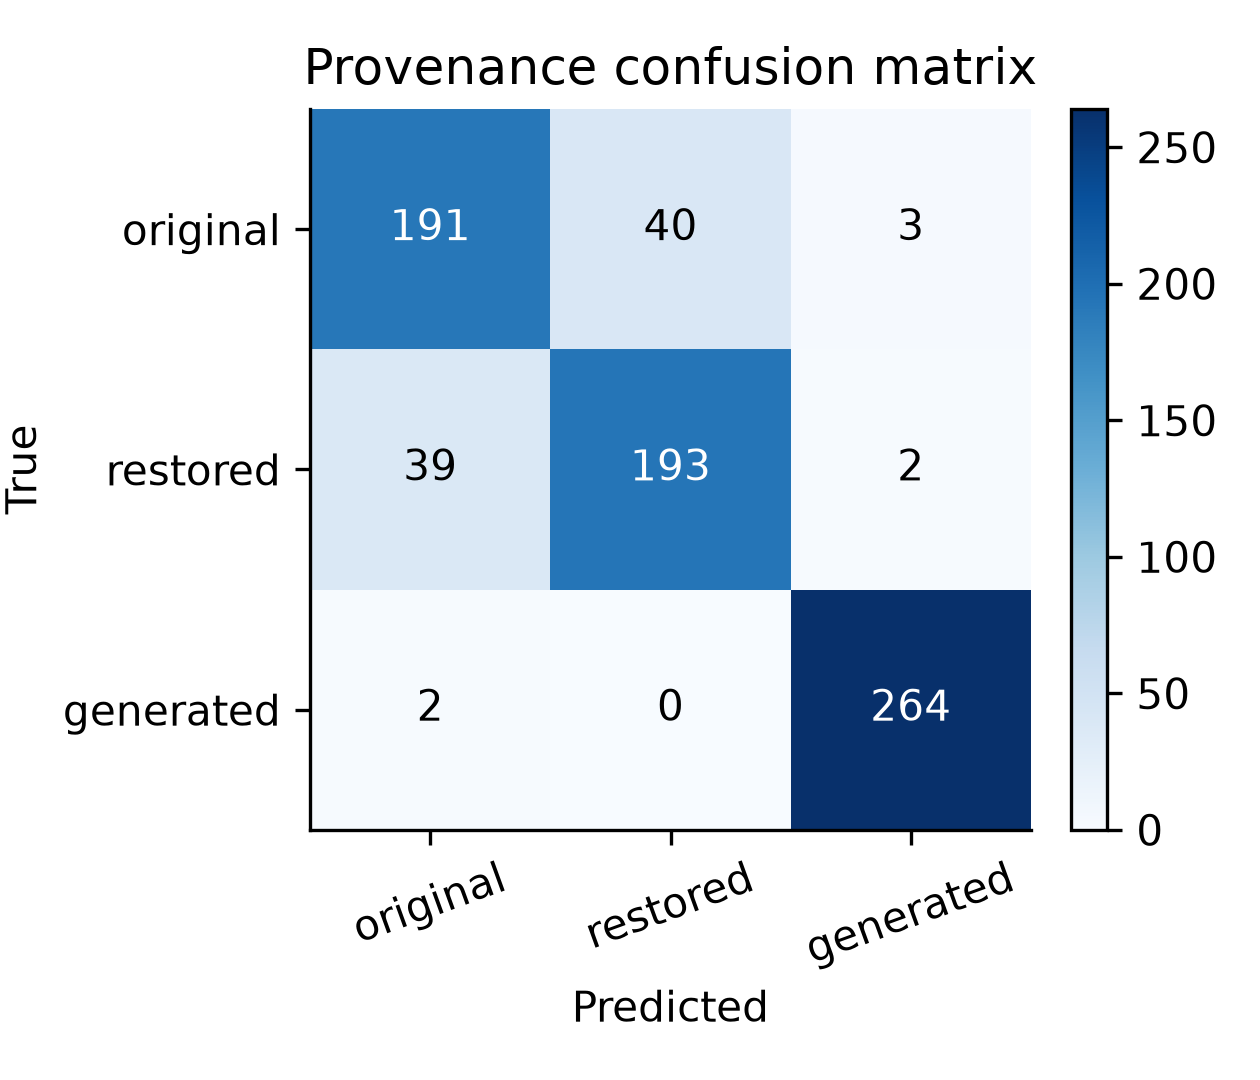
\includegraphics[width=0.46\textwidth]{figures/fig_confusion_matrix.png}
\caption{Confusion matrix at $224\times224$. Of 468 authentic test images, 79 are
confused between \emph{original} and \emph{restored}; only five authentic images are
predicted \emph{generated}.}
\label{fig:cm}
\end{figure}

The asymmetry is the central empirical fact of this study. Generated images are
almost perfectly separated, but the boundary that matters for authentic photographs
is not the real/fake boundary: it is the original/restored boundary. A detector
reported to be ``99\% accurate'' on a balanced binary benchmark says very little
about how it behaves on an authentic image that has been through a denoiser, because
that case does not appear in the benchmark.

\subsection{False-generated rate}
\label{sec:fpr}

Fig.~\ref{fig:fpr} plots the false-generated rate for original and restored
authentic images across the threshold range, and Table~\ref{tab:fpr} gives the
values at the conventional 0.5 operating point.

\begin{table}[t]
\centering
\caption{False-generated rate: share of authentic images whose predicted
probability for \emph{generated} reaches 0.5.}
\label{tab:fpr}
\begin{tabular}{@{}llrl@{}}
\toprule
Input & Condition & $n$ & Flagged as generated \\
\midrule
\multirow{2}{*}{$128\times128$} & original & 234 & 2.14\% [0.43, 4.27] \\
                                & restored & 234 & 0.85\% [0.00, 2.14] \\
\multirow{2}{*}{$224\times224$} & original & 234 & 1.28\% [0.00, 2.99] \\
                                & restored & 234 & 0.85\% [0.00, 2.14] \\
\bottomrule
\end{tabular}
\end{table}

\begin{figure}[t]
\centering
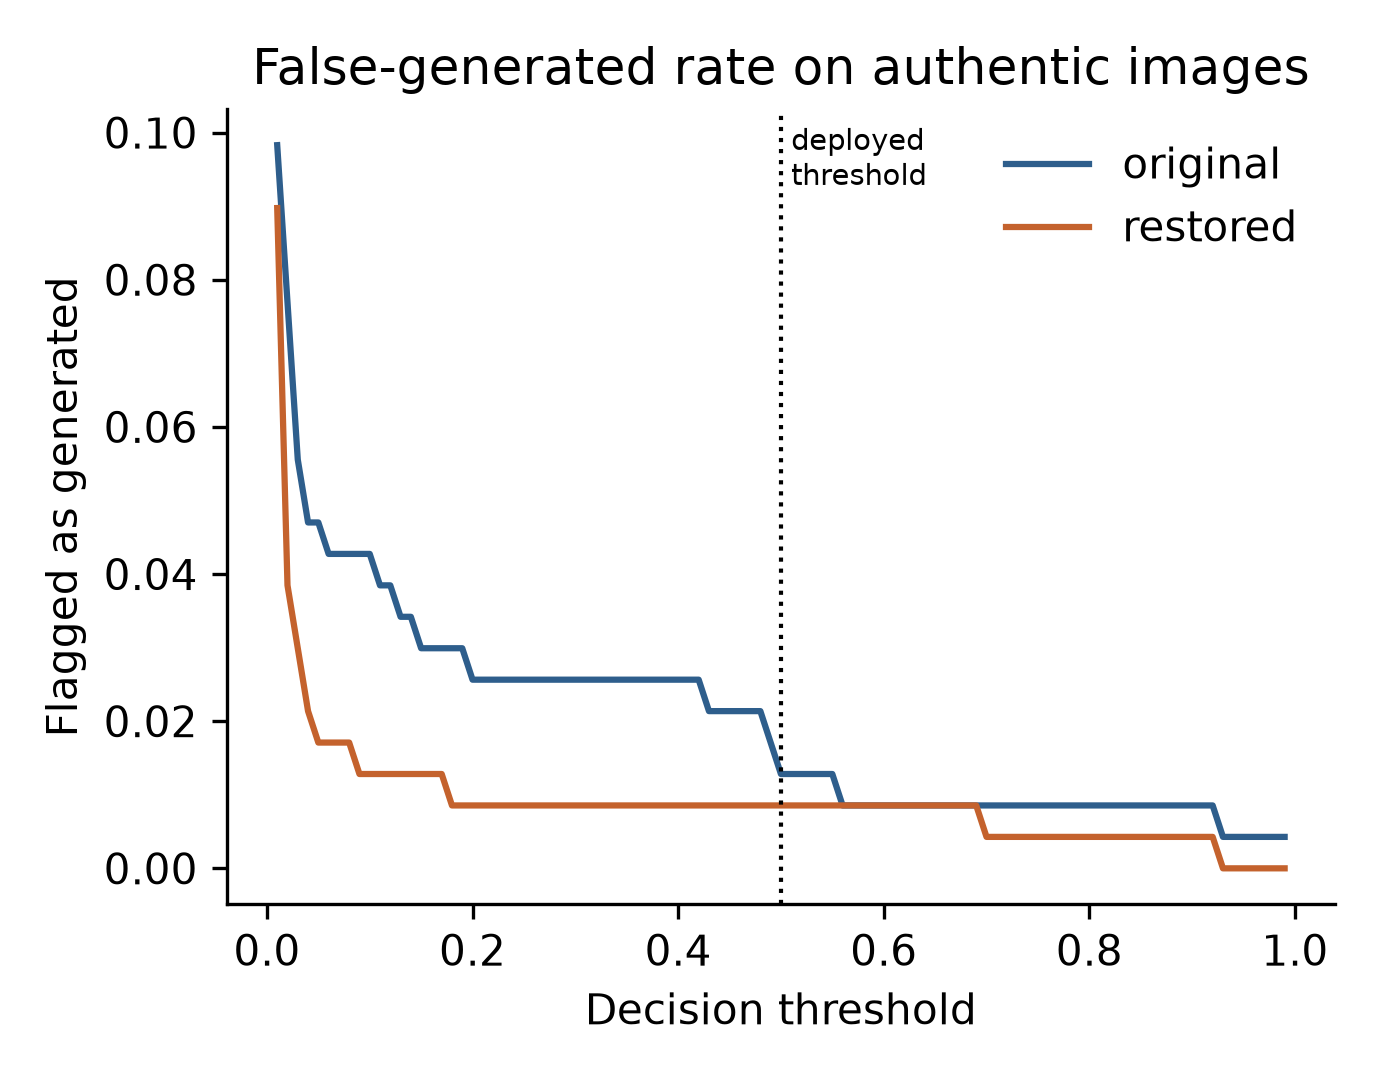
\includegraphics[width=0.52\textwidth]{figures/fig_fpr_threshold.png}
\caption{False-generated rate against the decision threshold at
$224\times224$. The restored curve lies below the original curve over the entire
range, so the ordering is not an artefact of the 0.5 operating point.}
\label{fig:fpr}
\end{figure}

Restoration does not increase the false-generated rate for this classifier. It
slightly decreases it, and the ordering holds across thresholds rather than only at
0.5. A binary real-versus-generated classifier trained only on \emph{original} and
\emph{generated} images shows the same pattern when applied to unseen authentic
photographs: 1.00\% false positives on pristine images and 0.30\% on their
restorations, with 96.60\% true positives on held-out generated images and AUROC
0.997.

We state the scope of this finding precisely. It is a property of a frozen
ImageNet ResNet-50 probe. The official-detector audit below shows why this
qualification matters: restoration is not universally detector-poisoning. The effect
depends on the detector, and a claim of the form
``restoration raises the false-positive rate from $x$ to $y$'' is meaningless
without naming the model, the threshold, and the restorer.

\begin{table}[t]
\centering
\caption{Official detector audit at threshold 0.5 on 1,000 paired images.}
\label{tab:official}
\begin{tabular}{@{}lrr@{}}
\toprule
Detector and restorer & Original & Restored \\
\midrule
CNNSpot (0.5), Real-ESRGAN & 0.30\% & 0.20\% \\
CNNSpot (0.5), Restormer & 0.30\% & 0.30\% \\
CNNSpot (0.1), Real-ESRGAN & 1.20\% & 0.90\% \\
CNNSpot (0.1), Restormer & 1.20\% & 1.70\% \\
UnivFD, Real-ESRGAN & 0.60\% & 1.60\% \\
UnivFD, Restormer & 0.60\% & 1.60\% \\
\bottomrule
\end{tabular}
\end{table}

The official runs do not reproduce the abstract's 15.90\% super-resolution or
5.20\% denoising rates. UnivFD rises from 0.60\% to 1.60\% for both restorers;
CNNSpot's released variants range from decreases to a 1.20\%--1.70\% rate.

\subsection{Generalisation to an unseen generator family}

We hold out one generator family entirely and train a binary real-versus-generated
classifier on the remaining three families plus authentic images.
Table~\ref{tab:unseen} gives the result.

\begin{table}[t]
\centering
\caption{Real vs.\ generated with one family unseen, $128\times128$.}
\label{tab:unseen}
\begin{tabular}{@{}lrr@{}}
\toprule
Unseen family & Accuracy & AUROC \\
\midrule
BigGAN & 98.27\% & 0.999 \\
VQDM   & 98.40\% & 0.998 \\
GLIDE  & \best{80.27\%} & \best{0.932} \\
ADM    & 88.00\% & 0.982 \\
\midrule
Mean AUROC & & 0.978 \\
\bottomrule
\end{tabular}
\end{table}

The mean of 0.978 is high, but the variance is the point. Two families transfer
above 0.998 and one drops to 0.932, a gap of six to seven accuracy points. GLIDE is
a text-guided diffusion model whose outputs differ in composition and texture
statistics from the GAN and quantised-diffusion families, and its lower transfer
matches the known difficulty of cross-family diffusion detection
\cite{corvi2023diffusion,ojha2023univfd}. Reporting the mean alone would present a
homogeneous capability that does not exist.

\section{Threats to Validity}
\label{sec:threats}

\paragraph{Content confound.} Authentic images are COCO photographs and generated
images are GenImage samples derived from ImageNet classes. A classifier can exploit
scene statistics and composition rather than synthesis artefacts, which inflates
generated recall and the original-versus-generated AUROC of 0.998. The
original-versus-restored contrast, AUROC 0.889, is immune to this confound because
both sides are the same photograph; we therefore weight it more heavily in our
conclusions. Removing the confound properly requires GenImage's matched real split or
a second authentic source drawn from the same distribution, which we did not run.

\paragraph{Detector checkpoint scope.} We ran the released CNNSpot Blur+JPEG(0.5)
and Blur+JPEG(0.1) checkpoints and the released UnivFD CLIP ViT-L/14 checkpoint.
Their results are an audit on this corpus, not an exact reproduction of the
abstract's rates: checkpoint version, preprocessing, corpus composition, and
restorer implementation all affect the measured false-positive rate.

\paragraph{One restorer per family.} Real-ESRGAN is the only super-resolution
operator and Restormer the only denoiser. We did not complete leave-one-restorer-out
transfer, so the results cannot establish generality across the restoration literature.

\paragraph{Resolution ceiling.} GenImage is 128\,px, so the matched comparison is at
128\,px and the standard comparison upsamples generated images by 1.75$\times$. Part
of the 224\,px gain reflects authentic detail that generated images do not have.

\paragraph{Single seed and single backbone.} We report one seed and one frozen
backbone. Variance across seeds is not quantified, and a CLIP or DINOv2 feature space
would likely change the absolute numbers, though not the qualitative split between
the two boundaries.

\section{Conclusion}

Provenance is not binary once restoration is in the pipeline. On a controlled
3{,}000-image corpus, a frozen ResNet-50 probe recovers original, restored, and
generated labels with 88.28\% accuracy and macro-AUROC 0.957, and the errors
concentrate on the original/restored boundary while generated images remain nearly
separable. Restoration is detectable from its own source photograph at AUROC 0.889,
which is far from the near-perfect separation of synthesised content but far from
chance. Cross-family transfer is strong on average and uneven in practice. Most
importantly, the false-positive inflation that motivates concern about restoration
did not appear for our classifier, which means it must be measured per deployed
detector rather than assumed from the presence of restoration. A provenance system
that names restoration as its own state turns a false accusation into a
recoverable provenance downgrade, and that is a better failure to have.

\subsubsection*{Data and code availability}
The corpus, manifest, trained head, prediction files, and the scripts that produce
every number and figure in this paper are included with the submission. The pipeline
rebuilds the corpus from public sources and retrains from scratch with fixed seeds;
no reported value is entered by hand.

\bibliographystyle{splncs04}
\bibliography{refs}

\end{document}
